\chapter{Die Analyse und Tests}
\label{cha:Analyse}
Dieses Kapitel beschäftigt sich mit der Analyse der Implementierung und dessen Tests. Es gibt zwei Arten von Tests die implementiert wurden
\begin{itemize}
	\item die \emph{JUnit}-Tests sind die Tests, die nicht auf eine \emph{CDI}-Umgebung angewiesen sind und 
	\item die \emph{CDI-JUnit}-Tests sind die Tests, die auf eine \emph{CDI}-Umgebung angewiesen sind.
\end{itemize}

\section{Die Tests}
Dieser Abschnitt beschäftigt sich mit den Implementieren Tests des Vorlagenmanagements und der Implementierten Konfiguration für die Tests. Für die Tests wurden folgende Bibliotheken verwendet.
\begin{itemize}
	\item\emph{JUnit4} ist ein \emph{Framework}, mit dem wiederholbare Tests implementiert werden können und ist als Standard für Tests in \emph{Java} anzusehen.
	\item\emph{Deltaspike} ist ein \emph{Open-Source}-Projekt der \emph{Apache Software Foundation (ASF)}, die portable \emph{CDI}-Erweiterungen in Form von Modulen bereitstellt und auch eine Erweiterung für \emph{JUnit}-Tests bereitstellt, mit denen Tests in einer \emph{CDI}-Umgebung lauffähig sind.
\end{itemize}
\ \newline
Alle implementierten Tests sind nicht auf einen Anwendungsserver angewiesen und sind innerhalb des lokalen Klassenpfades lauffähig und können daher in jeder Entwicklungsumgebung und bei einem Kompilieren über das \emph{Buildtool Maven} ausführbar.
\newline
\newline
Die Tests wurden wie folgt organisiert.
\begin{itemize}
	\item\emph{com.clevercure.mailing.test.*} 
	\newline
	ist das \emph{Java}-Paket in dem alle implementierten Tests liegen. 
	\item\emph{*.[toTestClass]Tests}
	\newline
	ist das \emph{Java}-Paket, für eine zu testende Klasse, wobei der Paketname den Namen der zu testenden Klasse mit dem Suffix Tests enthält.
	\item\emph{[toTestMethod]Test.java}
	\newline
	ist die implementierte Testklasse für die Tests einer Methode der zu testenden Klasse.
	\item\emph{test\_case}
	\newline
	ist der Name der einzelnen Testmethoden, der wiedergibt was an einer Methode getestet wird. 
\end{itemize}
\ \newline
Die vorgestellte Konvention der Tests wurde so umgesetzt sofern es möglich war. 

\subsection{Die Tests der \emph{CDI}-Erweiterung}
Die Tests aus Abbildung \ref{fig:tests-template-cdi} testen die Implementierungen des Artefakts \emph{mailing-moule-template-cdi} wie
\begin{itemize}
	\item die Klasse \emph{TemplateCdiExtension},
	\item die Klasse \emph{CdiTemplateUtils} und
	\item die Klasse \emph{TemplateResourceProducer}.
\end{itemize}
\begin{figure}[h]
\centering
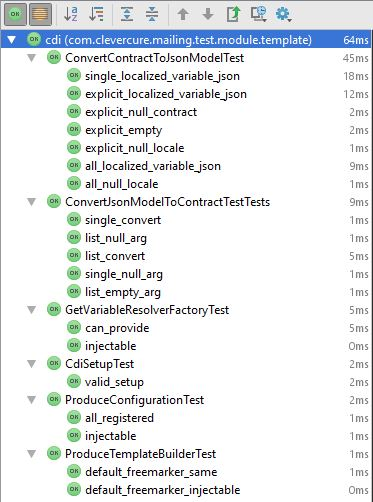
\includegraphics[scale=0.7]{tests-template-cdi}
\caption{Testdurchlauf der Tests der \emph{CDI}-Erweiterung}
\label{fig:tests-template-cdi}
\end{figure}
Diese Tests sind nur lauffähig in einer \emph{CDI}-Umgebung, die aber Dank \emph{Deltaspike} auch im Klassenpfad ohne Anwendungsserver gestartet werden kann. Im Klassenpfad der Tests wurde Variablen über eine \emph{Enumeration}, die die Schnittstelle \emph{VariableContract} implementiert, definiert, sowie eine Implementierung der Klasse \emph{VariableResolverFactory}.

\subsection{Die Tests des implementierten \emph{FacesConverters}}
Die Tests der \emph{JSF}-Integration testen den implementierten \emph{FacesConverter}, der die Voralgen von ihrer \emph{HTML}-Repräsentation in die \emph{Freemarker}-Repräsentation konvertiert.
\begin{figure}[h]
\centering
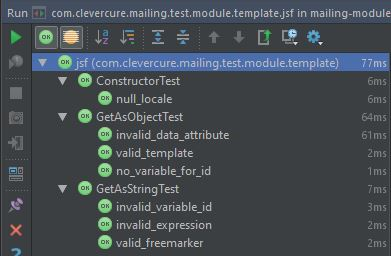
\includegraphics[scale=0.7]{tests-template-jsf}
\caption{Testdurchlauf der Tests des \emph{FacesConverters}}
\label{fig:tests-template-jsf}
\end{figure}
\ \newline
Obwohl die Schnittstelle \emph{FacesConverter} aus \emph{JSF} kommt, ist es nicht notwendig eine \emph{JSF}-Umgebung zu starten.

\subsection{Die Tests des implementierten Vorlagenmanagements}
Die Tests aus Abbildung \ref{fig:tests-template-impl} testen die Implementierungen der Logik des Vorlagenmanagements. Die Logik ist in den beiden Klassen 
\begin{itemize}
	\item die Klasse \emph{VariableConfigurationImpl} und
	\item die Klasse \emph{FreemarkerTemplateDataJsonBuilder} implementiert.
\end{itemize}
\ \newline
Diese Tests sind nicht abhängig von einer \emph{CDI}-Umgebung. Es wird getestet ob Variablen korrekt registriert werden und in einem Objekt der Klasse \emph{VariableConfigurationImpl} korrekt verwaltet werden und ob die Klasse \emph{FreemarkerTemplateDataJsonBuilder} in der Lage ist ein Objekt der Klasse \emph{TemplateRequestJson} zu produzieren, dass die Daten für eine Voralge hält.
\newpage
\begin{figure}[h]
\centering
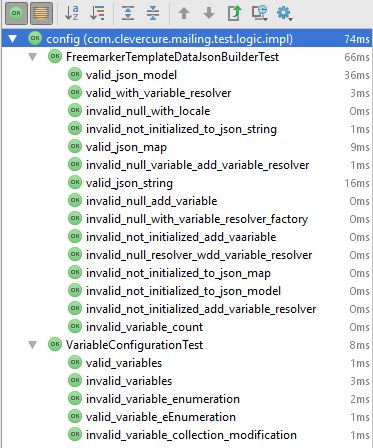
\includegraphics[scale=0.7]{tests-template-impl}
\caption{Testdurchlauf der Tests des Vorlagenmanagement}
\label{fig:tests-template-impl}
\end{figure}
\ \newline
Diese Tests sind nicht angewiesen auf eine \emph{CDI}-Umgebung und sind ohne zusätzliche Bibliotheken und \emph{Framwork} lauffähig. Sie Testen die implementierten Methoden und vor allem bezüglich derer Fehlerbehandlung.

\section{Die erreichten Ziele}
Dieser Abschnitt beschäftigt sich mit der Betrachtung der erreichten Ziele des implementierten Vorlagenmanagements. Es wurden alle Anforderung aus dem Kapitel \ref{cha:Zielsetzung} erfüllt, somit gilt das Vorlagenmanagement als abgeschlossen. Die Integrationen in die Anwendungen \emph{CleverWeb} und \emph{CleverInterface} wurde noch nicht realisiert, obwohl begonnen wurde eine Integration für die Anwendung in \emph{CleverWeb} zu implementieren. Die Integration in die Anwendung \emph{CleverInterface} wird erst realisiert werden können, wenn diese Anwendung \emph{Java} in Version 8 unterstützt. Zurzeit wird nur \emph{Java} in version 7 unterstützt. 

\subsection{Das Vorlagenmanagement über das \emph{CKEditor-Plugin}}
Es wurde erfolgreich ein \emph{Plugin} in \emph{Typescript} für den \emph{CKEditor} implementiert, dass das Variablenmanagement des Vorlagenmanagements erfolgreich \emph{Browser} seitig in den \emph{CKEditor} integriert. Wie in Abschnitt \ref{sec:sub-typescript-javascript} behandelt, wurde das \emph{Plugin} in \emph{Typescript} umgesetzt und das \emph{CKEditor-Plgun} von dem Variablenmanagement getrennt und in eigenen Quelltextdateien implementiert. Die implementierten \emph{Typescript}-Quelltexte befinden sich zurzeit noch in der Demowebanwendung, da die Entwicklung in einem eigenen Projekt nicht möglich war, da das \emph{Hot-Code-Deployment} für \emph{Java}-Ressourcen (src/main/resources) nicht unterstützt wird. Diese Quelltextdateien können einfach in ein anderes Projekt verschoben werden. Die Quelltextdateien werden jetzt noch über die Entwicklungsumgebung kompiliert, kann aber in Zukunft über das \emph{Maven-Plugin maven-grunt-plugin} auch automatisiert bei jedem \emph{Build} kompiliert werden. 

\subsection{Das Vorlagenmanagements in \emph{CDI}}
Es wurde erfolgreich die Integration des Vorlagenmanagement in eine \emph{CDI}-Umgebung implementiert. Die in Abschnitt \ref{sec:sub-impl-integartion-cdi} behandelte Integration in eine \emph{CDI}-Umgebung, wurde über eine portierbare \emph{CDI}-Erweiterung realisiert, die beim Start der \emph{CDI}-Umgebung alle implementierten Klassen der Schnittstellen \emph{VariableContract (enum)} und \emph{VariablenResolver} findet, registriert und über die Anwendungsdauer verwaltet. Diese gesammelten Ressourcen werden kontextabhängig zur Verfügung gestellt und können über Injektion in ein Objekt injiziert werden.

\subsection{Das Vorlagenmanagement in \emph{JSF}}
Es wurde erfolgreich eine Integration in \emph{JSF} implementiert, wobei diese Integration über einen \emph{FacesConverter} erreicht wurde, der die Vorlagen von ihrer \emph{HTML}-Repräsentation in die \emph{Freemarker}-Repräsentation konvertieren kann. Wie in Abschnitt \ref{sec:sub-impl-integartion-jsf} vorgestellt, wurde die gemeinsame Logik in einer abstrakte Klasse \emph{AbstractTemplateConverter} gekapselt, der nur bekanntgegeben werden muss, welche konkrete Implementierung, definiert über eine Qualifizierer Annotation, genutzt werden soll. Über diese abstrakte Klasse wird sichergestellt, dass die \emph{HTML}-Repräsentation der Variablen über alle \emph{Template-Engines} gleich ist.

\subsection{Das Vorlagenmanagement in \emph{Mail}-DB-Schema}
Die Integration der Vorlagen in des \emph{Mail-DB}-Schema war die die einfachste Aufgabe, da hier lediglich eine einfache Datenstruktur definiert werden muss, die in der Lage ist, die Vorlagen mehrsprachig persistent zu halten. Prinzipiell ist eine Vorlage auf einer Datenbank als Zeichenkette präsent, wobei nur auf die Größe der Zeichenkette geachtet werden muss.
